\section{Sequence State Diagram}

\subsection{Cosa sono gli SSD?}
Un diagramma di sequenza di sistema (SSD) è un diagramma UML che mostra gli eventi in input e output dei sistemi in discussione
\subsection{Quali sono gli obiettivi di un SSD?}
L'obiettivo principale della creazione di un SSD è comprendere le interazioni che sono implicate e descritte nei casi d'suo

\vspace{\baselineskip}

Il diagramma serve per visualizzare in modo immediato le funzioni e il comportamento del sistema con un approccio a "scatola nera", il suo scopo è descrivere che cosa fa il sistema in risposta agli stimoli esterni, omettendo e senza spiegare come lo fa al suo interno
\subsection{Perchè disegnare gli SSD?}
Disegnare gli SSD è cruciale perchè gli eventi di sistema sono fondamentali per l'architettura del software, il quale deve essere progettato esattamente per gestire tali eventi

\vspace{1\baselineskip} \noindent

Utilizzando la notazione UML, serve a illustrare le interazioni tra gli attori e il sistema.

\subsection{Componenti degli SSD}

\subsubsection{Attori Esterni}
\begin{center}
    \begin{tikzpicture}
        \umlactor{Attore}
    \end{tikzpicture}
\end{center}

Rappresentano le persone o entità che interagiscono direttamente con il sistema. Il loro ruolo è quello di partecipare allo scenario generando gli eventi (input).

\vspace{1\baselineskip} \noindent


Il loro ruolo è quello di partecipare allo scenario generando gli eventi (input) per richiedere al sistema l'esecuzione di specifiche operazioni.

\vspace{1\baselineskip} \noindent

Per distinguere visivamente un attore umano da un attore che è un sistema informatico, si usa spesso la dicitura «actor» all'interno di un rettangolo per quest'ultimo

\subsubsection{Il Sistema}

\begin{center}
    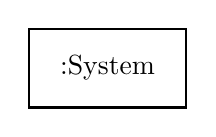
\begin{tikzpicture}
        \draw[thick] (0,0) rectangle (2,1) node[pos=.5] {:System};
    \end{tikzpicture}
\end{center}

Viene rappresentato come un'unica entità indivisibile (spesso etichettata graficamente con :System).

\vspace{1\baselineskip} \noindent

La sua funzione nel diagramma è quella di mostrare che cosa fa il sistema ricevente in risposta agli input, ma omettendone volutamente i processi interni su come lo fa (da qui il termine "scatola nera").

\vspace{1\baselineskip} \noindent



\subsubsection{Eventi di sistema}
\begin{center}
    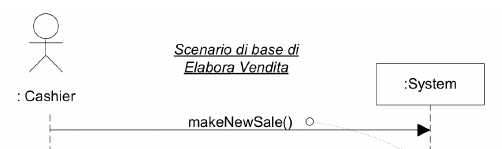
\includegraphics{figures/Schermata_20260425_173900.png}
\end{center}

\vspace{1\baselineskip}
Sono eventi esterni generati dagli attori per richiedere un'operazione di sistema e sono disposti seguendo il loro preciso ordine cronologico.

\vspace{\baselineskip}

Sono eventi esterni generati dagli attori e sono disposti seguendo il loro preciso ordine cronologico.

\vspace{\baselineskip}

Graficamente appaiono come linee continue a forma di freccia e possono includere l'invio di parametri,

\vspace{\baselineskip}

I nomi di questi eventi rappresentano un'intenzione astratta e dovrebbero iniziare con un verbo.

\subsubsection{Valori di ritorno}
\begin{center}
    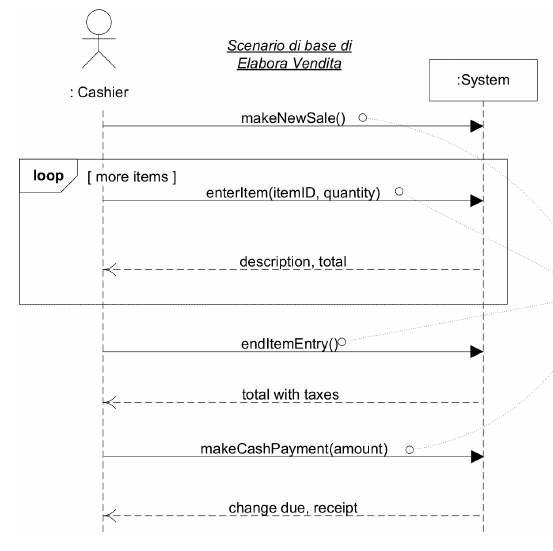
\includegraphics{figures/Schermata_20260425_174843.png}
\end{center}


Sono le risposte o le informazioni che il sistema produce e rimanda all'attore in seguito all'elaborazione di un evento.

Vengono tracciati utilizzando una linea tratteggiata, si tratta di una componente opzionale che pu essere omessa nel caso in cui l'operazione non restituisca niente

\subsubsection{Frame di interazione}
\begin{center}
    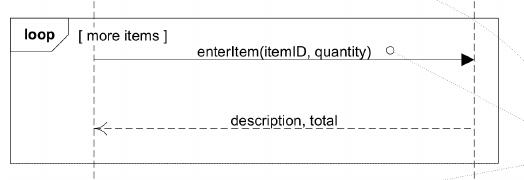
\includegraphics{figures/Schermata_20260425_175324.png}
\end{center}
Sono costrutti grafici a forma di riquadro utilizzati per raggruppare e strutturare specifiche parti dell'interazione

\subsubsection{Sistemi esterni (ed eventi inter-sistema)}
\begin{center}
    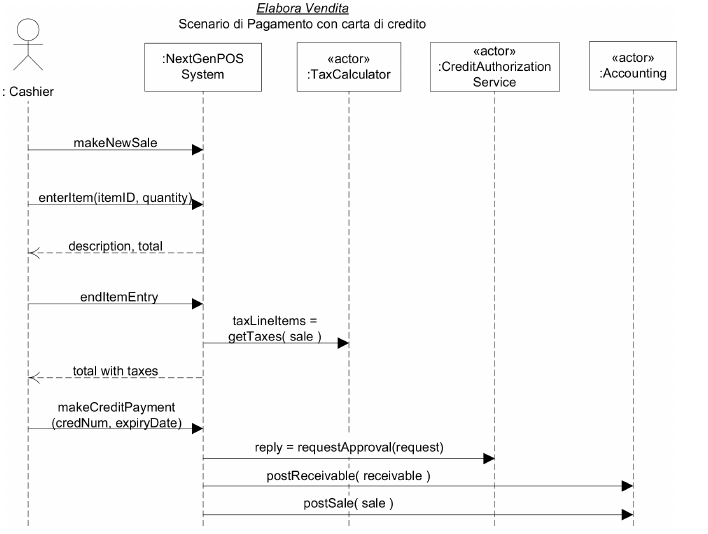
\includegraphics{figures/Schermata_20260425_175606.png}
\end{center}
Qualora lo scenario preveda che il sistema debba delegare operazioni ad altri enti informatici, il diagramma includerà la rappresentazione di questi attori-sistemi aggiuntivi e mostrerà le interazioni necessarie con essi

\subsection{Relazione con gli altri elaborati UML}
L'SSD non è un elaborato isolato, ma si inserisce all'intero del processo UP in strettissima relazione con gli altri documenti dell'analisi e della progettazione, fungendo da "ponte" tra i requisiti testuali e la progettazione vero e propria

\subsubsection{Casi d'Uso}
Gli SSD fanno formalmente parte del Modello dei casi d'uso.

\vspace{\baselineskip}

Mentre i casi d'uso descrivono il compoeramento e i requisiti in forma testuale, l'SSD prende un particolare scenario e ne visualizza graficamente le interazioni implicate

\subsubsection{Contratti delle Operazioni di Sistema}
La relazione è di stretta dipendenza procedurale, si parte dall'SSD per poter creare i contratti.

\vspace{\baselineskip}

Le frecce di input (eventi di sistema) che vanno dall'attore verso il sistema nell'SSD rappresentano la richiesta di esecuzione di un'operazione di sistema.

Il primissimo passo per scrivere i contratti è proprio "identificare operazioni di sistema dagli SSD"

\vspace{\baselineskip}

Una volta individuate, per le operazioni più complesse si scrivere un contratto che descrive dettagliatamente come lo stato del sistema cambierà a seguito di quell'evento

\subsubsection{Glossario}
Poichè un SSD è un diagramma grafico, i nomi delle operazioni, i parametri inviati e i valori restituiti sono scritti in modo estremamente coinciso.

Affinchè non ci siano ambiguità durante la successiva fase di progettazione su "cosa entra e cosa esce", la linea guida prevede che tutti i dettagli di questi elementi sintetici dell'SSD vengano spiegati in modo approfondito nel Glossario

\subsubsection{Modello di Dominio}
L'SSD si collega al Modello di Dominio attraverso gli eventi che genera.

\vspace{\baselineskip}

L'esecuzione di'un operazione di sistema ha lo scopo di cambiare lo stato del sistema, e questo stato è rappresentato proprio dagli oggetti presenti nel modello di Dominio.

\vspace{\baselineskip}

Inoltre, analizzando gli eventi dell'SSD per scrivere i contratti, è del tutto normale accorgersi di dover aggiornare il Modello di Dominio, registrando nuove classi concettuali, associazioni o attributi che prima non erano emersi

\section{Contratti delle operazioni di sistema}
\subsection{Cosa sono i Contratti delle Operazioni di Sistema?}
I contratti delle operazioni di sistema sono documenti che descrivono il comportamento del software in modo molto più dettagliato rispetto a quanto facciano i casi d'uso.

\vspace{\baselineskip}

Mentre un caso d'uso racconta una storia, il contratto si concentra su un singolo evento di input (un'operazione) e definisce con precisione quali cambiamenti quello specifico evento provoca all'interno del sistema (ovvero agli oggetti del modello di dominio)

Tutto questo viene fatto mantenendo un approccio a "scatola nera", il contratto descrive i risultati finiali dell'operazione, senza mai spiegare la logica interna usata per ottenerli

\subsubsection{Cosa è un operazione di sistema?}
Un'operazione di sistema è una trasformazione o un'interrogazione pubblica che il sistema viene chiamato a eseguire per gestire un evento in unput generato da un attore esterno

\vspace{\baselineskip}

\begin{itemize}
    \item \textbf{È una reazione a un evento:}
    \begin{quote}
        Un'operazione di sistema non parte mai da sola. 
        
        La sua esecuzione è sempre richiesta da un evento di sistema.
    \end{quote}

    \item \textbf{Modifica lo stato del sistema:}
    \begin{quote}
        Quando viene eseguita, un'operazione cambia lo stato del software.
        
        In fase di analisi, questo cambiamento si traduce graficamente nello stato degli oggetti presenti nel Modello di Dominio.
    \end{quote}

    \item \textbf{Costituisce l'interfaccia del sistema :}
    \begin{quote}
        L'insieme di tutte le operazioni di sistema pubbliche definiscono l'intera interfaccia del software, ovvero l'elenco esatto di "tutto ciò che il sistema sa fare" in risposta agli stimoli esterni
    \end{quote}
\end{itemize}

\subsection{Struttura dei Contratti}

\vspace{\baselineskip}

\begin{center}
    % Aumenta lo spazio tra le righe per non schiacciare il testo
    \renewcommand{\arraystretch}{1.5} 

    \begin{tabularx}{\textwidth}{ l | X }
        \multicolumn{2}{c}{\textbf{Nome Contratto}} \\ \hline
        \textbf{Operazione} & \textit{Nome dell'operazione e parametri} \\
        \hline
        \textbf{Riferimenti} & \textit{casi d'uso correlati} \\
        \hline
        \textbf{Pre-condizioni} & \textit{Ipotesi sullo stato del sistema prima dell'operazione} \\
        \hline
        \textbf{Post-condizioni} & \textit{Cambiamenti di stato dopo l'operazione (scritte al passato)} \\
    \end{tabularx}
\end{center}

\vspace{\baselineskip}

La struttura di un contratto delle operazioni di sistema si divide in 4 sezioni principali : 

\vspace{\baselineskip}

\begin{enumerate}
    \item \textbf{Operazione : } Indica il nome e i parametri, ovvero la firma dell'operazione
    \item \textbf{Riferimenti : } Specifica i casi d'uso all'interno dei quali questa operazione può verificarsi
    \item \textbf{Pre-Condizioni : } Descrive le ipotesi significative e non banali relative allo stato del sistema, o degli oggetti presenti nel Modello di Dominio, prima che l'operazione venga eseguita.

    Questa sezione funge da sintesi dello stato di avanzamento del caso d'uso e serve a comunicare al lettore quali informazioni il sistema deve necessariamente già conoscere o aver soddisfatto
    \item \textbf{Post-Condizioni : } È considerata la sezione più importante del contratto e descrive i cambiamenti che sono avvenuti nello stato degli oggetti all'interno del Modello di Dominio che l'operazione è stata completata.
    
    \vspace{\baselineskip}

    Le dichiarazioni in questa sezione non devono descrivere le azioni interne eseguite dal sistema, ma unicamente i risultati ottenuti

    \vspace{\baselineskip}

    Inoltre, devono essere scritte rigorosamente con un verbo al passato e rientrare sempre in una di queste 3 caterie di cambiamento :
        \indent 
        \begin{enumerate}[label = \arabic*., leftmargin=1.5cm]
            \item La creazione o cancellazione di un oggetto
            \item La modifica del valore di un attributo
            \item La formazione o rottura di un collegamento
        \end{enumerate}
\end{enumerate}

\subsection{Relazione con gli altri elaborati UML}
I contratti delle operazioni di sistema hano una stretta relazione di interdipendenza con gli altri elaborati del processo UP e di UML

\vspace{\baselineskip}

Fanno formalmente parte del Modello dei casi d'uso e fungono da ponte tra l'analisi dei requisiti e la progettazione vera e proprio del software 

\subsubsection{Casi D'uso}
I contratti sono complementari ai casi d'uso.

\vspace{\baselineskip}
Mentre i casi d'uso descrivono il comportamente e i requisiti del sistema in forma testuale e generale, i contratti intervengono per descrivere in modo molto più dettagliato situazioni complesse che non sarebbe opportuno o pratico inserire normalmente nel normale testo del caso d'uso.

Non a caso, la struttura del contratto prevede una sezione "Riferimenti" che indica esplicitamente in quale caso d'uso si verifica l'operazione

\subsubsection{Diagrammi SSD}
La creazione dei contratti dipendi proceduralmente dagli SSD.

\vspace{\baselineskip}

Il primo passo operativo per scrivere i contratti consiste proprio nell'identificare le operazioni di sistema guardando gli SSD.

L'SSD mostra l'evento di sistema generato dall'attore, e il contratto entra nel dettaglio di come quell'operazione invocata cambi lo stato del sistema

\subsection{Modelli di Dominio}
Il legame è fortissimo, i contratti utilizzano le pre-condizioni e post-condizioni unicamente per descrivere i cambiamenti agli oggetti presenti all'interno del Modello di Dominio.

\subsection{OCL - Object Constraint Language}
Nell'ecosistema UML, un'operazione ha una firma ed è associata a un insieme di vincoli per specificarne la semantica.

In teoria, i vincoli descritti nel contratto possono essere espressi in modo rigorosamente formale avvalendosi dell'OCL, un linguaggio nato in UML appositamente per questo scopo